\begin{frame}{Biomas}
    \begin{itemize} \setlength\itemsep{1em}
        \item Conceito de biomas usado por \cite{walter1986vegetaccao};
        \item O conceito de biomas utilizado neste trabalho.
    \end{itemize}
    \begin{figure}
        \centering
        \begin{subfigure}[b]{0.47\textwidth}
            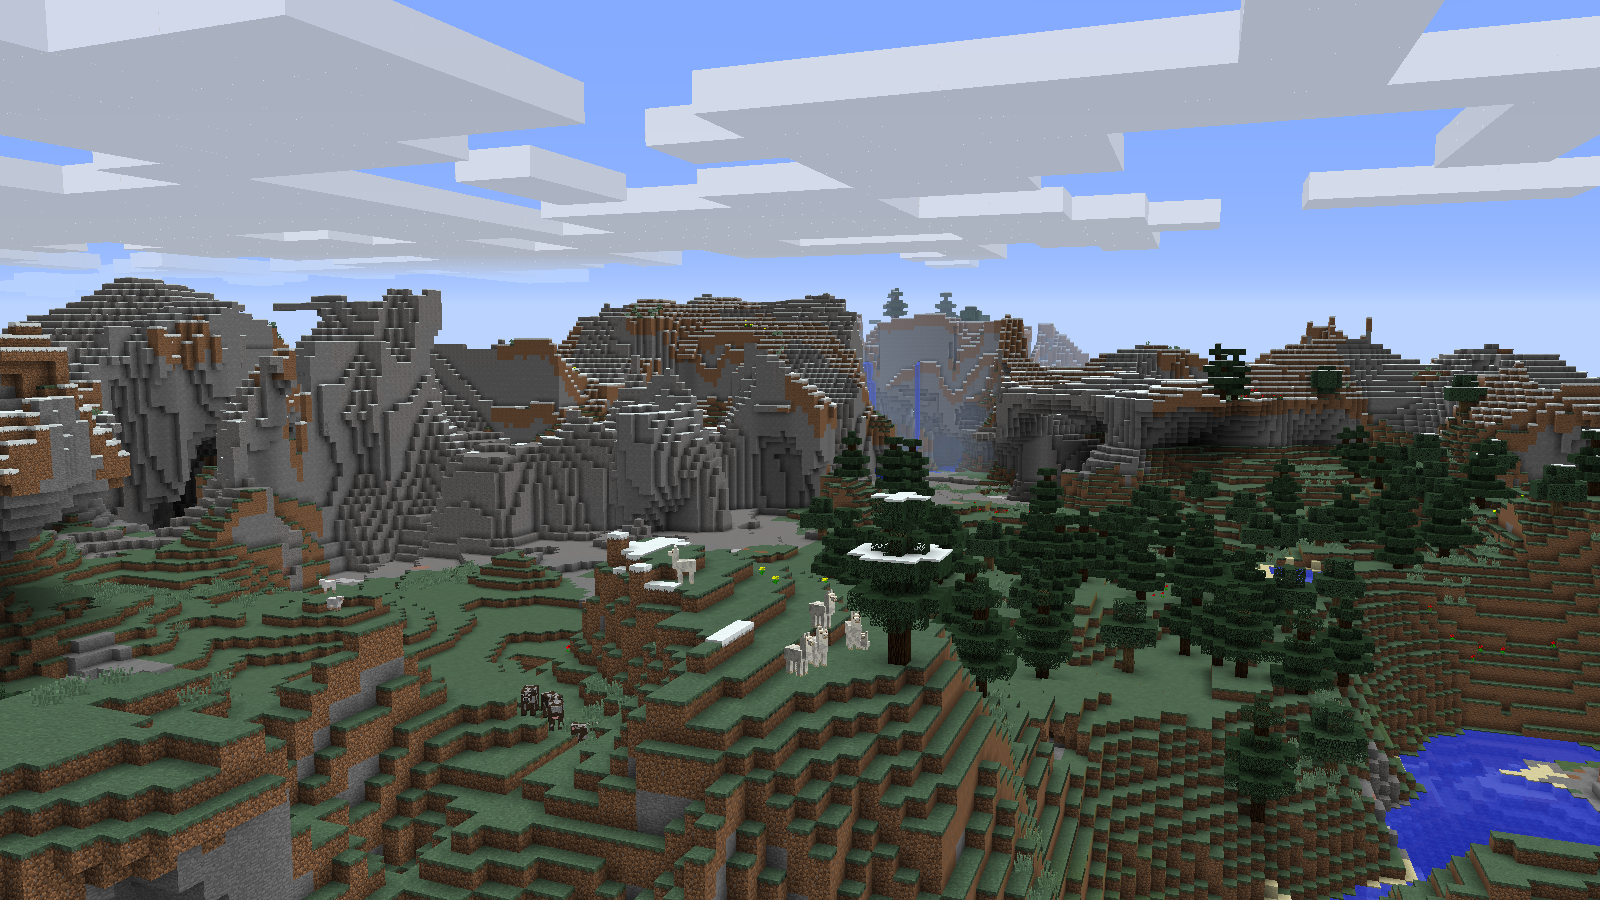
\includegraphics[width=\textwidth]{img/mineExtremeHills}
            \caption{Bioma \textit{Extreme Hills} no minecraft}
            \label{fig:mineExtremeHills}
        \end{subfigure}
        ~ %add desired spacing between images, e. g. ~, \quad, \qquad, \hfill etc. 
          %(or a blank line to force the subfigure onto a new line)
        \begin{subfigure}[b]{0.47\textwidth}
            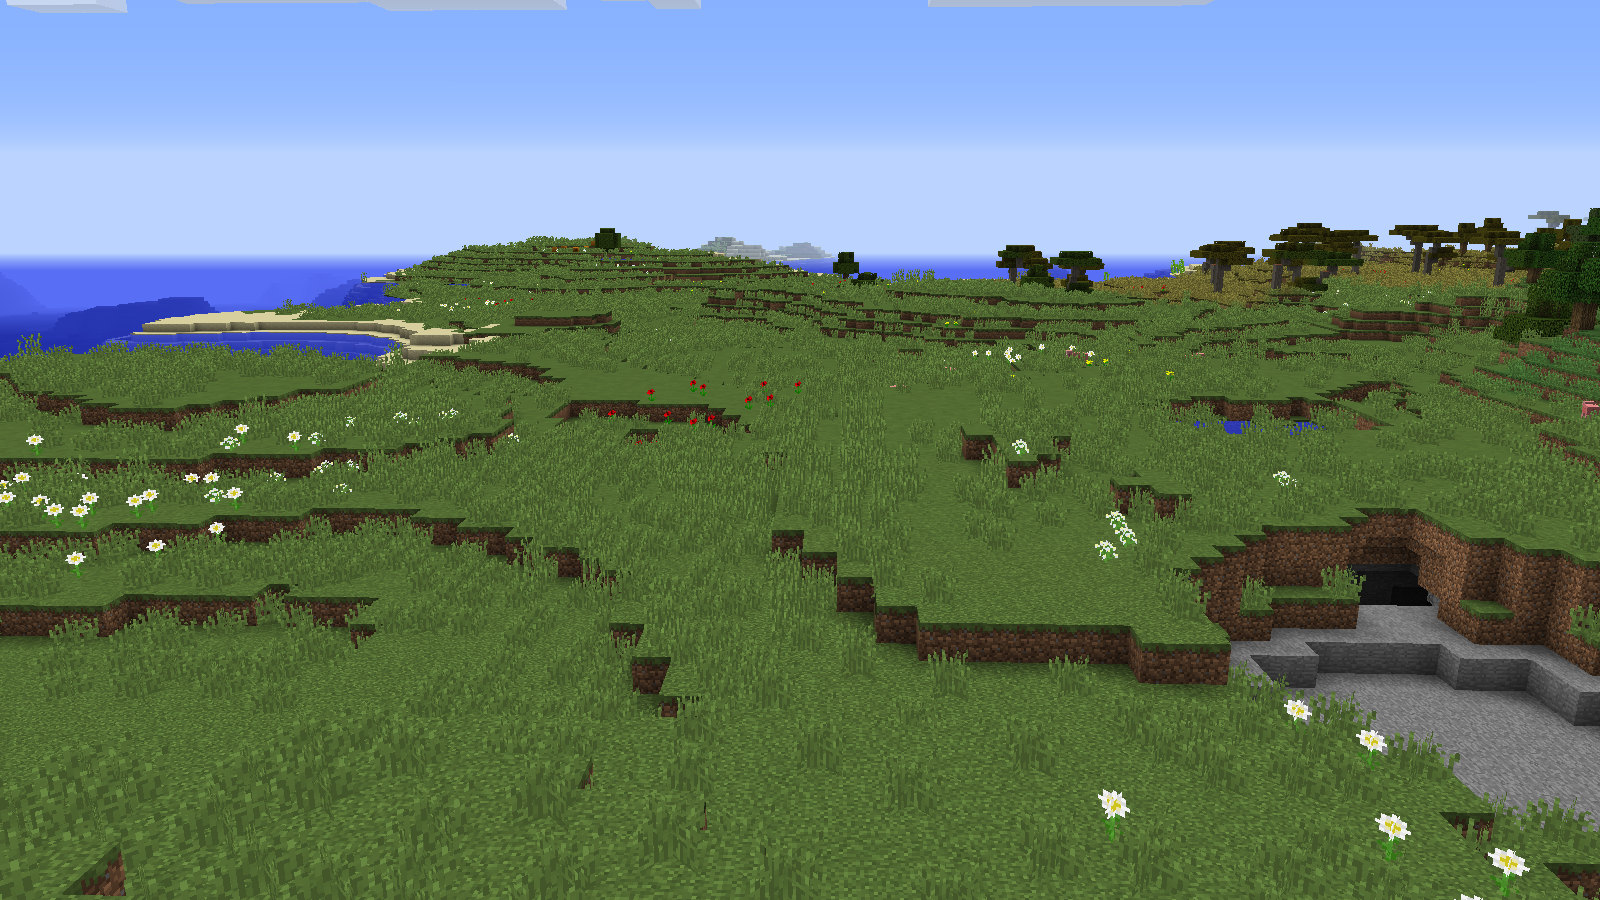
\includegraphics[width=\textwidth]{img/minePlains}
            \caption{Bioma \textit{Plains} no minecraft}
            \label{fig:minePlains}
        \end{subfigure}
        ~ %add desired spacing between images, e. g. ~, \quad, \qquad, \hfill etc. 
        %(or a blank line to force the subfigure onto a new line)
        \caption{Exemplo de Biomas no minecraft}
        \label{fig:mineBiomes}
    \end{figure}
    
    
\end{frame}